\chapter{Search by Snapを用いたユーザ実験}
\label{chapter:experiment_sbs}
本章では,Search by Snapを用いて実施したユーザ実験と,その結果について述べる.
\section{実験の目的}
  \ref{section:searching_action}節で述べたように,慣れていない地域や周囲の文字が読めないに状況おいて,ユーザが目の前にある店舗の情報や条件に合致する店舗の情報を瞬時に取得することは容易ではない.
  位置情報を手がかりに周囲の検索を行い,条件に合った店舗が見つかったとしても,ユーザ自身が居る環境と検索行為とが分断されているため,そのその環境からその店舗を探す手間が残るという問題点がある.
  そのため,提案システムを用いることによって,位置情報を利用したサービスと比較して店舗を簡単かつ直感的に探索できることを確認する.
  本稿では,地域に慣れていないユーザを対象に評価を行う前段階として,提案システムのユーザビリティを評価するために,地元の大学生を対象にユーザ実験を実施する.

\section{予備実験}
  \subsection{実験の概要}
    実験は大阪府高槻市にある高槻本通りにおいて,曇りの日の昼間において,\ref{chapter:implement_sbs}章で実装したシステムを用いて店舗を探索する際のユーザの行動の観察するために,ユーザが商店街において条件に合う店舗を探している状況を想定して行なった.
    実験参加者は情報系の学部に通う大学生4名である.

    表\ref{table:storelist}に示す15店舗を対象とし,実験参加者にはタスク(1)として,支払いにVISAカードが使える店舗を探すこと,タスク(2)として,月曜日の24時以降に営業している店舗を探すこと,の2点を課した.
    それぞれ提案システムを用いた場合とWeb検索エンジンを用いた場合とで探索に要した時間及び正確さを測定した.
    Web検索エンジンには,World Wide Web上で最も多く使われている検索エンジン\cite{Alexa:2019}であるGoogle検索\footnote{\url{https://www.google.com}(2019/2/1存在確認)}を用いる.
    実験に用いる端末は,\ref{chapter:experiment_dr}章と同じNexus 7である.
    
  \subsection{実験の手順}
    探索に用いる手法の順序効果によるデータの偏りを排除するため,実験は2人同時に行い,タスク(1)は1人が提案システムを用いて行い,もう1人がGoogle検索を用いて行う.
    2人がタスク(1)を終えたら,実験参加者はタスク(2)を異なる手法を用いて行う.

    実験の手順として,初めに,実験参加者に回答用フォームのURLを伝え,参加者は自身のスマートフォンでフォームを開く.
    次に,提案システムの操作方法を実験参加者に説明する.
    その後,2人の実験参加者が同時に探索を開始し,フォーム上で条件に合致する店舗のチェックボックスを選択する.
    実験参加者が探索を開始してから送信ボタンをタップするまでの時間を測定する.
    
    実験終了後には,参加者に「求めていた情報の見つけやすさ(簡便性)」,「情報探索の直感性(直感性)」について,提案システムとGoogle検索との間で5段階のリッカート尺度を用い,「1」を「Google検索」,「5」を「提案システム」として5段階評価のアンケートへの回答を求めた.

  \subsection{実験の結果と考察}
    実験の結果を図\ref{figure:exp_sbs_pre_result}に示す.
    探索時間に関しては,システムを用いた場合はGoogle検索を用いた場合と比較して短くなる傾向が見られた.
    正確さに関しては,システムを用いた場合とGoogle検索を用いた場合とで差は見られない傾向があった.
    アンケートの結果を表\ref{table:exp_sbs_pre_questionnaire}に示す.
    アンケートの結果から,提案システムを用いることによって,Google検索を用いた場合より直感的かつ簡易に探索ができるようになることが示唆された.

    \begin{figure}[t]
      \begin{minipage}{0.49\hsize}
        \begin{center}
          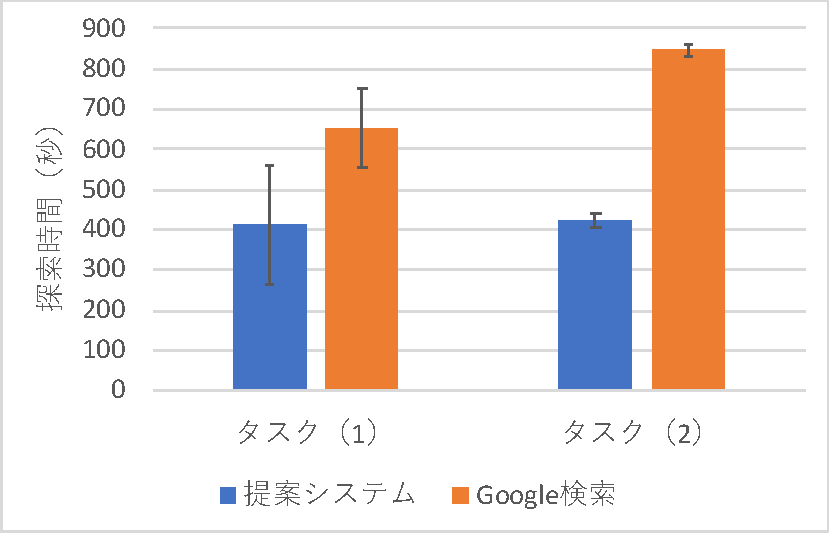
\includegraphics[clip, width=\textwidth]{sbs_pre_result_time.pdf}\\
          \small{(a)探索時間}
        \end{center}
      \end{minipage}
      \begin{minipage}{0.49\hsize}
        \begin{center}
          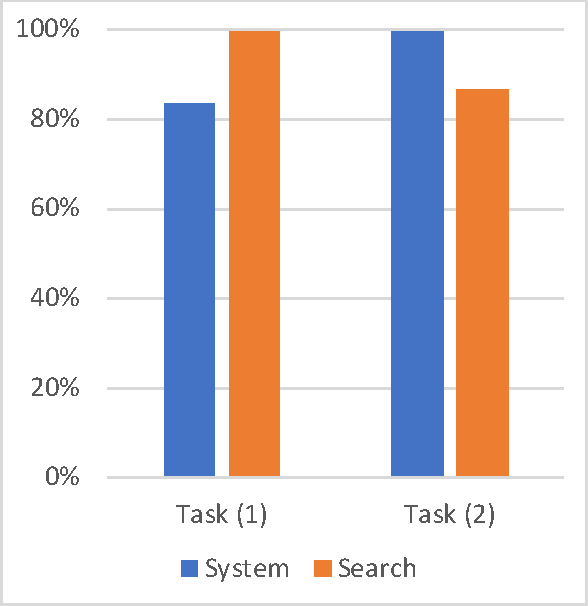
\includegraphics[clip, width=\columnwidth]{sbs_pre_result_acc.pdf}
          \small{(b)正解率}
        \end{center}
      \end{minipage}
      \caption{予備実験の結果}
      \label{figure:exp_sbs_pre_result}
    \end{figure}

    \begin{table}
      \begin{center}
        \caption{予備実験のアンケート結果}
        \label{table:exp_sbs_pre_questionnaire}
        \begin{tabular}{c|ccp{9cm}}
          \hline \hline
          \textbf{実験参加者} & \textbf{簡便性} & \textbf{直感性} & \multicolumn{1}{c}{\textbf{コメント}} \\
          \hline
          A & 5 & 5 & カメラを向けるだけですぐ情報が見えるのでよかった \\
          B & 5 & 5 & 看板を映してパッと求めている情報が出てくるのはとても良いなと思いました。情報が見つけやすい。 \\
          C & 4 & 5 & 同じ地域に何店舗もある店だと検索サイトで検索した際、どの店かわかりづらく時間がかかりました。 \\
          D & 5 & 4 & \\
          \hline
        \end{tabular}
      \end{center}
    \end{table}

  \subsection{ユーザ観察}
    実験中のユーザを観察した結果,システムを用いて探索する際,至近距離で看板を認識しようとする行動が見られた.端末のカメラが店舗の看板の大部分の領域を捉えられない場合,正常に看板を認識できない場合が多いため,本実験では看板から一定の距離を置いて端末のカメラを向けるよう指示を与える.Google検索を用いて探索する際,多くのユーザがタスク(1)においては「(店舗名) 高槻」というクエリ,タスク(2)においては「(店舗名) 高槻 営業時間」というクエリで検索を行っていた.対象がチェーン店である場合,位置に関する情報をクエリとして与えなければ目的の情報に素早く辿り着けず,探索に時間を要している傾向が見られた.多くのユーザは,対象が飲食店である場合においては,Google検索結果に表示された食べログのサイトへ移動し,そこから情報を得ていた.そのため,本実験では,探索対象を飲食店に限定し,食べログを用いて提案システムとの比較を行う.

\section{本実験}
  \subsection{実験の概要}
    実験は大阪府高槻市にある高槻本通りにおいて,昼間にユーザが飲食店を探している状況を想定して行った.
    実験参加者は情報系の学部に通う大学生10名である.

    実験参加者にはタスク(A)として,「小だるま JR高槻駅前店」,「肉丼専門店 高槻肉劇場」,「磯丸水産 高槻店」の3店舗について,使用できるクレジットカードの種類を``Visa'',``Mastercard'',``JCB'',``American Express'',``Diners Club''の5つのチェックボックスから全て選択すること,タスク(B)として,「おだいどこはなれ 高槻店」,「高槻ちゃぶちゃぶ」,「赤から 高槻店」の3店舗について,月曜日の営業開始時刻を数値で入力すること,の2点を課した.
    タスク(A)は図\ref{figure:exp_sbs_point}中\textcircled{\scriptsize 1}で示した位置に立った状態,タスク(B)は図\ref{figure:exp_sbs_point}中\textcircled{\scriptsize 2}で示した位置に立った状態で行った.
    実験に用いた携帯端末はクアンタ・コンピュータ社\footnote{http://www.quantatw.com}のVA-10J(Android 5.0.2)である.
    提案システムとの比較対象とする位置情報を用いたサービスは,ランキングやユーザの口コミ・写真をもとにレストランの検索が行えるサービスである食べログ\footnote{https://tabelog.com}を用いた.

  \begin{figure}[tb]
    \begin{center}
      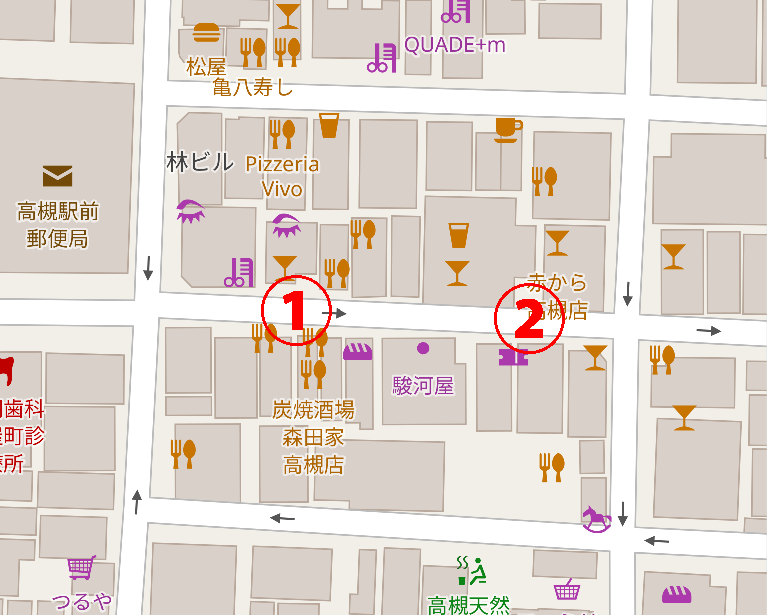
\includegraphics[clip, width=.95\columnwidth]{sbs_map_point.pdf}
      \caption{実験の実施地点}
      \label{figure:exp_sbs_point}
    \end{center}
  \end{figure}

  \begin{figure}[tb]
    \centerline{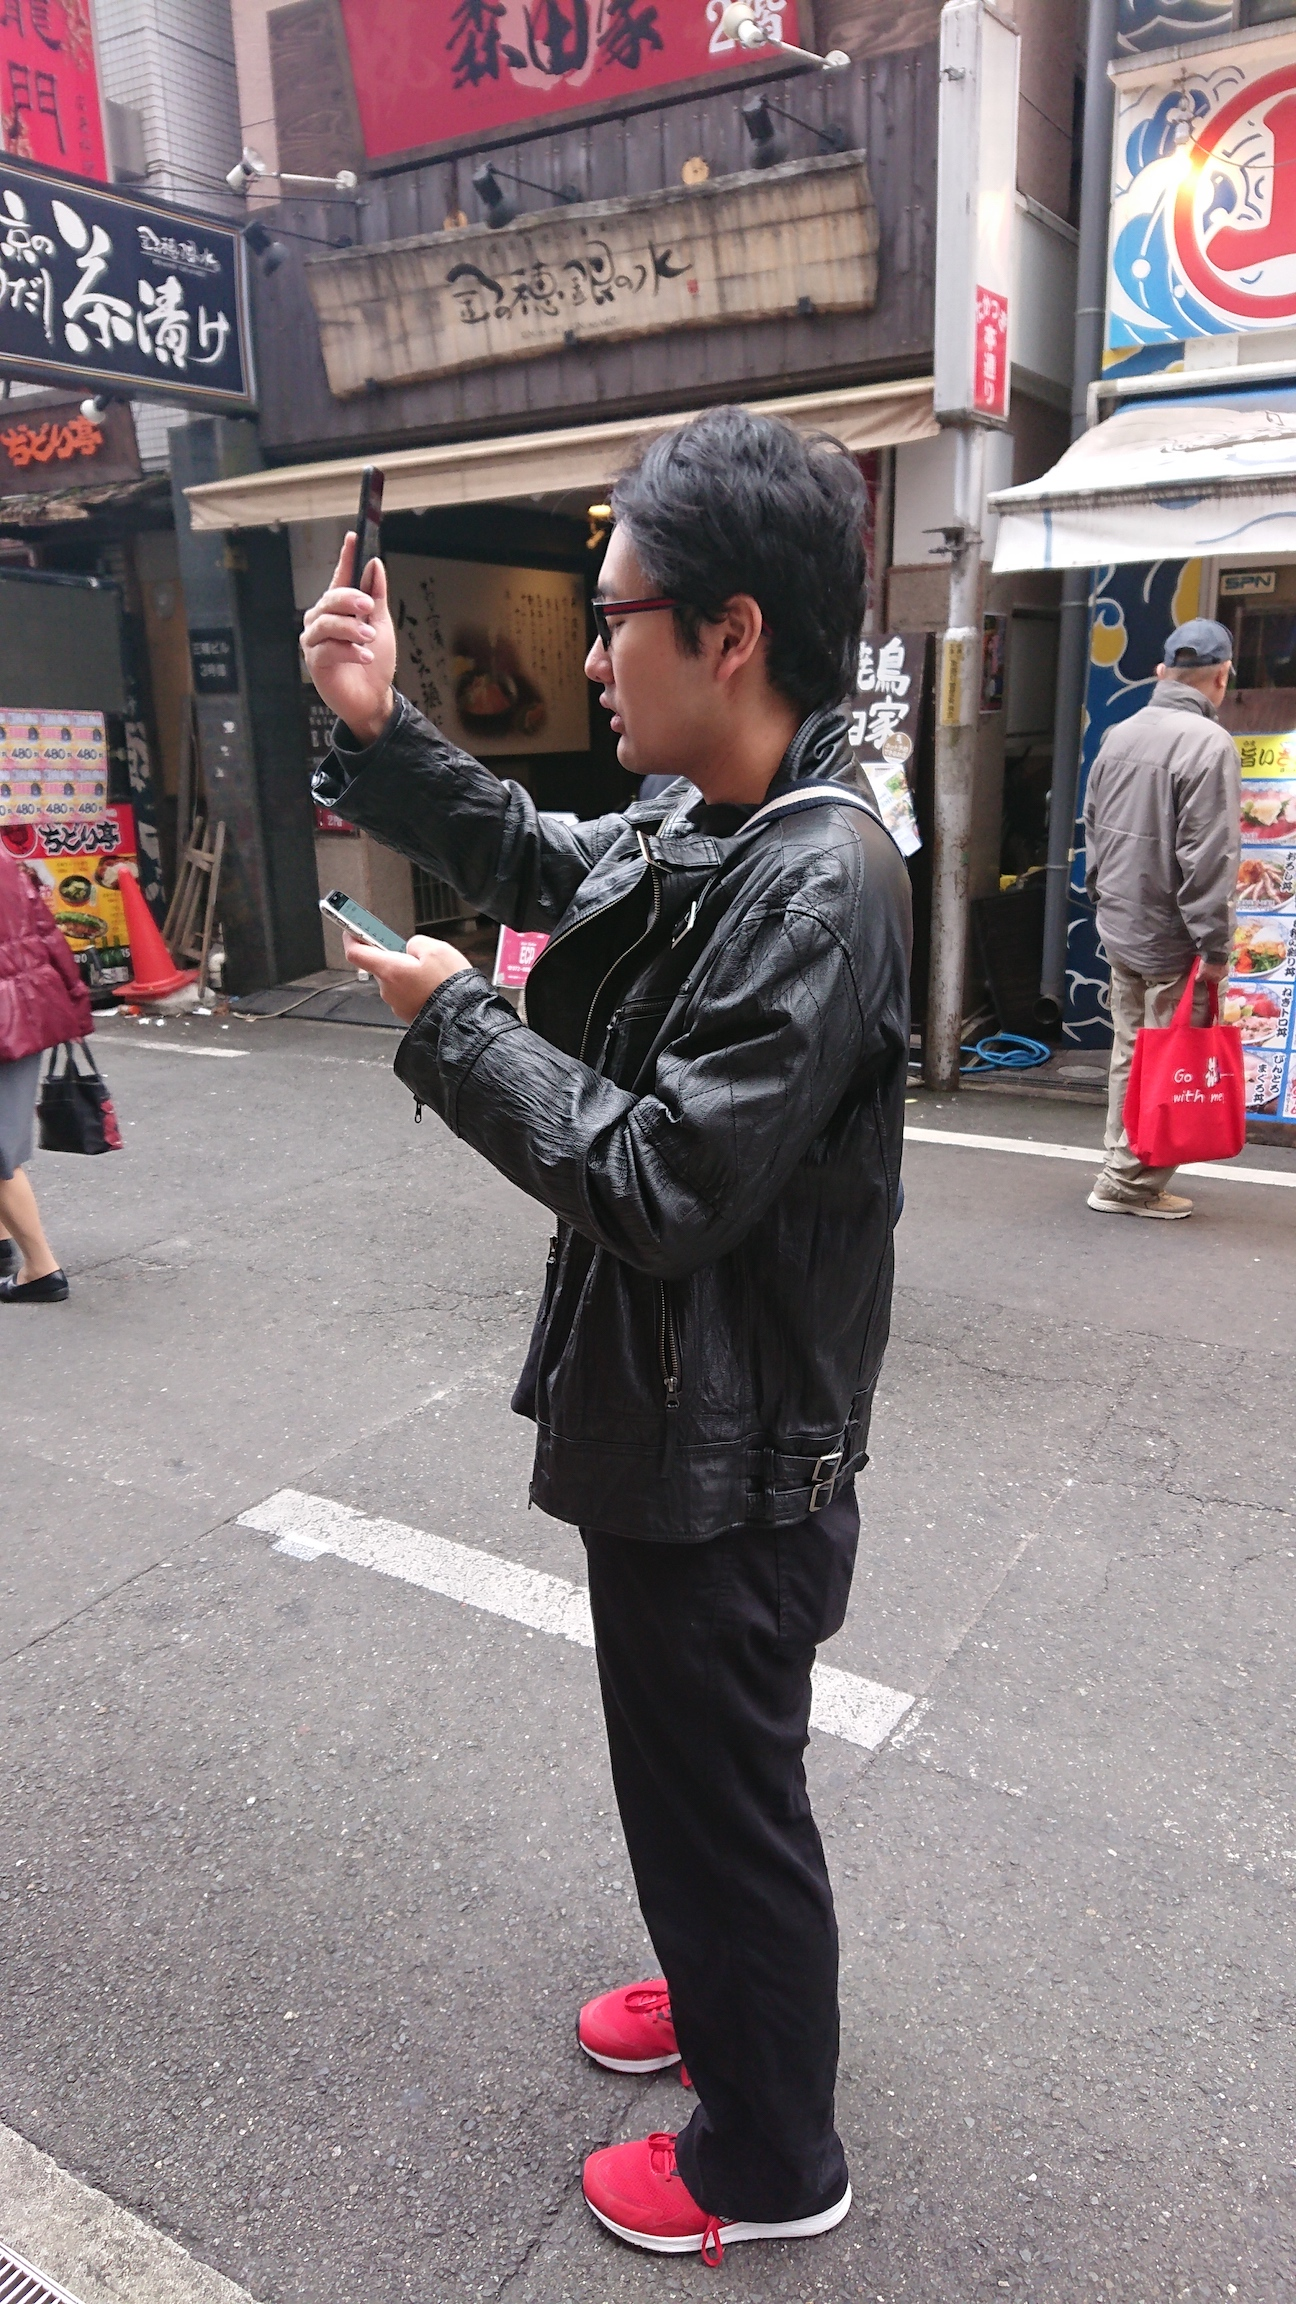
\includegraphics[width=.5\columnwidth, clip]{sbs_exp_scenery.jpg}}
    \caption{実験の風景}
    \label{figure:exp_sbs_scenery}
  \end{figure}

  \subsection{実験の手順}
    初めに,提案システムと食べログの使い方を実験参加者に説明する.
    次に,実験参加者に回答用フォームのURLを伝え,参加者は自身のスマートフォンでフォームを開く.
    実験に用いるシステムを起動した状態で参加者に実験用のスマートフォンを渡す.
    実験参加者はシステムを用いて求められている情報を探索し,フォームに入力して送信する.
    実験参加者がシステムの操作を始めてから送信ボタンをタップするまでの時間を計測する.
    実験の風景を図\ref{figure:exp_sbs_scenery}に示す.

    実験参加者をグループ(1)とグループ(2)に2分割し,グループ(1)にはタスク(A)を提案システム,タスク(B)を食べログを用いて行うよう指示を出し,グループ(2)にはタスク(A)を食べログ,タスク(B)を提案システムを用いて行うよう指示を出した.
    実験終了後には,参加者に「求めていた情報の見つけやすさ(簡便性)」,「情報探索の直感性(直感性)」について,食べログと提案システムとの間で5段階評価のアンケートへの回答を求めた.

  \subsection{実験の結果}
    実験参加者がシステムに操作を初めてから指示された情報を全て収集し,送信ボタンをタップするまでの時間を計測し,タスク(A)とタスク(B)に関して提案システムを用いた場合と食べログを用いた場合とにおいて,探索時間の平均値を比較した.その結果を図\ref{figure:exp_sbs_result_time}に示す.
    タスク(A)において,提案手法を用いた場合の探索時間は食べログを用いた場合よりも有意に短い($t(8)=2.343, p<.05$)ことが確認された.
    タスク(B)においても,提案手法を用いた場合の探索時間は食べログを用いた場合よりも有意に短い($t(8)=4.370, p<.05$)ことが確認された.

    各タスクにおいて,ユーザが正確に情報を収集できたかを測定するために,対象とした3店舗のうち,正確に情報を取得できた店舗数の割合を正解率として測定し,提案システムを用いた場合と食べログを用いた場合とにおいて,正解率の平均値を比較した.その結果を図\ref{figure:exp_sbs_result_acc}に示す.
    タスク(A)において,提案手法を用いた場合と食べログを用いた場合とで,正解率に有意差は見られなかった($t(8)=1.000, n.s.$).
    タスク(B)においても,提案手法を用いた場合と食べログを用いた場合とで,正解率に有意差は見られなかった($t(8)=1.633, n.s.$).

    予備実験と同様に,実験終了後に情報探索の簡便性と直感性について5段階のリッカート尺度を用い,「1」を「食べログ」,「5」を「提案システム」として5段階で回答してもらった.
    そのアンケート結果を表\ref{table:exp_sbs_questionnaire}に,アンケート結果の分布を図\ref{figure:exp_sbs_result_question}に示す.
    簡便性に関する平均値は4.4,直感性に関する平均値は4.5であった.

    \begin{figure}[tb]
      \begin{center}
        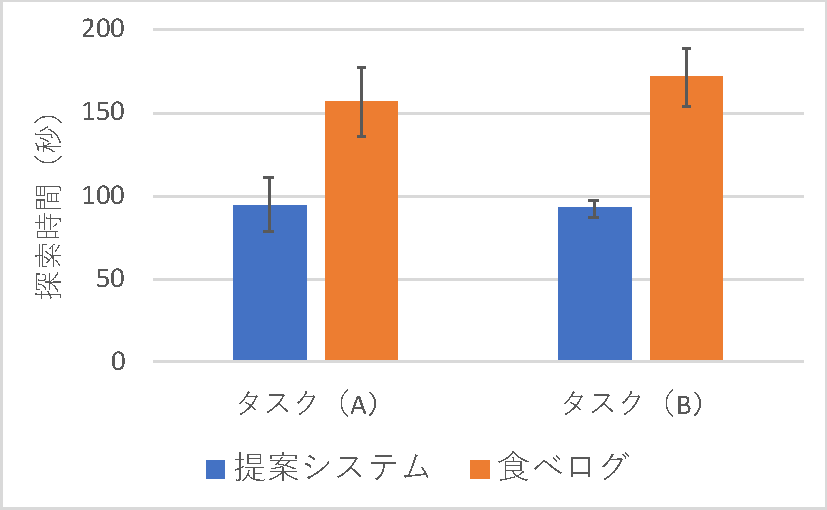
\includegraphics[clip, width=.95\columnwidth]{sbs_result_time.pdf}
        \caption{探索時間}
        \label{figure:exp_sbs_result_time}
      \end{center}
      \vspace{1cm}
      \begin{center}
        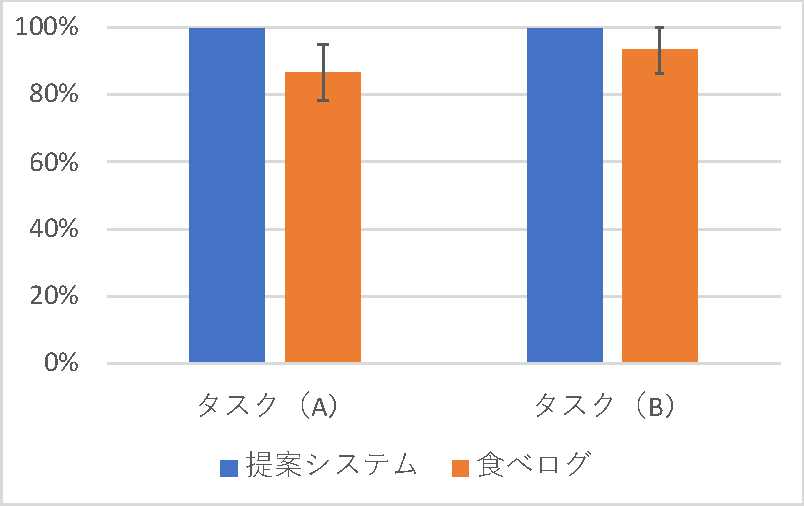
\includegraphics[clip, width=.95\columnwidth]{sbs_result_acc.pdf}
        \caption{正解率}
        \label{figure:exp_sbs_result_acc}
      \end{center}
    \end{figure}

    \begin{table}
      \begin{center}
        \caption{本実験のアンケート結果}
        \label{table:exp_sbs_questionnaire}
        \begin{tabular}{c|cccp{8cm}}
          \hline \hline
          \textbf{実験参加者} & \textbf{群} & \textbf{簡便性} & \textbf{直感性} & \multicolumn{1}{c}{\textbf{コメント}} \\
          \hline
          1  & A & 5 & 5 & 看板が多いところだと情報の表示が重なり見にくいところがあった。 \\
          2  & A & 4 & 4 & どちらの検索機能も分かりやすいと思います。 \\
          3  & A & 5 & 5 & リアルタイムな情報が検索できたらもっと便利かと思いました。 \\
          4  & A & 2 & 4 & システムを使った時に店の情報が違う店の情報に被ってしまって見にくいときがあったことと、情報が一定の場所に出続けないてなくて毎回情報と、店名とを見比べる必要がありました \\
          5  & A & 4 & 4 & 食べログはUI次第でどうにかなると思いました。 システムの方は、文字を色分けなどしていただいた方が目につきやすいのかとおもいました。 \\
          6  & B & 5 & 5 & タップ数やかかる時間でもシステムの方が有利に感じた。 \\
          7  & B & 5 & 4 & システムでは、欲しい店舗の情報を常に表示し続けるためには かざし続けなければいけなく、ズレてしまった場合 違う店舗情報が出てしまったため 慣れが必要なのかなと思いました。一方、食べログ検索では店舗によって載ってる情報がバラバラなため、必要な情報がなかった際に 本当に情報が無いのかのダブルチェックを必要とすることが億劫であった。 \\
          8  & B & 5 & 5 &  \\
          9  & B & 5 & 4 &  \\
          10 & B & 4 & 5 & すぐに情報を知れて便利だと思いました。 \\
          \hline
        \end{tabular}
      \end{center}
    \end{table}    

    \begin{figure}[tb]
      \begin{center}
        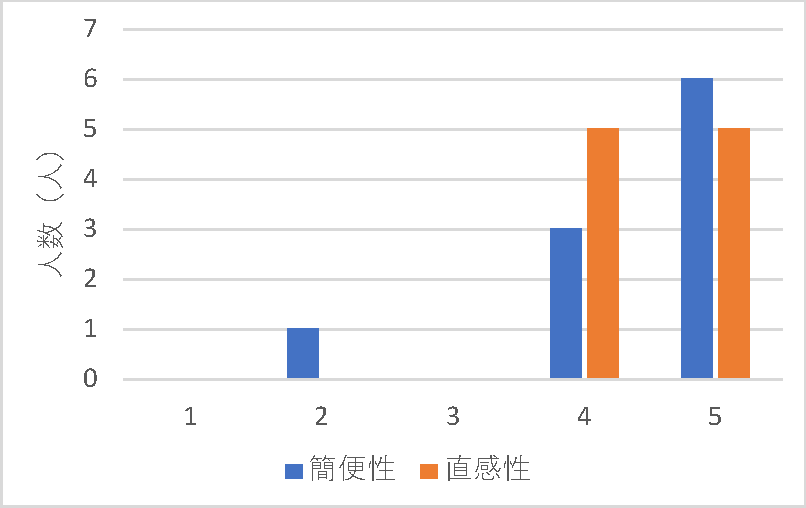
\includegraphics[clip, width=.95\columnwidth]{sbs_result_question.pdf}
        \caption{本実験のアンケート結果の分布(1: 食べログ〜 5: 提案システム)}
        \label{figure:exp_sbs_result_question}
      \end{center}
    \end{figure}